\documentclass[a4paper, 12pt, twoside, openright]{mythesis}
\usepackage[utf8]{inputenc}
% \renewcommand{\baselinestretch}{1}       % for squeezing the draft into the page limit, do not use

% Note
% Use \textsc{Name} to separate images, videos, dataset names from the main texts.

% =============================================================================
% Commonly used packages
% =============================================================================

% For removing Package ifpdf Error
%%%%%%\let\ifpdf\relax

% For removing LaTeX Font Warning
\usepackage{lmodern}

% Add Reference in Contents
\usepackage[nottoc]{tocbibind}

% Figures
%\usepackage{subcaption}
\usepackage{float}
\usepackage{adjustbox}
%\usepackage[justification=raggedright]{caption}	% makes captions ragged right - thanks to Bryce Lobdell
\usepackage{lscape} % Useful for wide tables or figures.
\usepackage{makecell}
\usepackage{sidecap}

\graphicspath{{figures}{example}}

% % Algorithm
% \usepackage[lined,ruled,linesnumbered]{algorithm2e}
% \usepackage{algorithmic}

% Table and list
\usepackage{booktabs} % Publication quality tables
\usepackage{multirow}
\usepackage{rotating} % sideways
\newcommand{\vergap}[1]{\renewcommand{\arraystretch}{#1}}
\newcommand{\horgap}[1]{\setlength{\tabcolsep}{#1}}
%\specialrule{width}{abovespace}{belowspace}
\newcommand{\dtoprule}{\specialrule{2pt}{0pt}{2pt}}
\newcommand{\dbottomrule}{\specialrule{2pt}{0pt}{\belowrulesep}}

\usepackage{paralist}
\usepackage{enumitem}

% Math and Physics
\usepackage{bm} % Make bold, italic math symbols
\usepackage{epsfig} % for figures
\usepackage{graphicx} % another package that works for figures
\usepackage{subcaption}
\usepackage{times}
%\usepackage{mathptmx}
\usepackage{mathtools}
\usepackage{textcomp, gensymb} % math symbol
\usepackage{amssymb,amsmath,amsfonts} % Short math guide for LaTeX ftp://ftp.ams.org/pub/tex/doc/amsmath/short-math-guide.pdf
\usepackage{siunitx} % SI units
\usepackage{physics}
\usepackage{feynmp-auto}
% \newcommand{\norm}[1]{\left\lVert#1\right\rVert}
% \newcommand{\cp}[1]{\left[#1\right]_{\times}}

% Fonts
\usepackage{units}
\usepackage{color}

% Comments
\usepackage{comment}

% Hyperlinks
\usepackage{url} % Hyphenation of URLs.
\usepackage{xcolor}
\usepackage[backref=page]{hyperref}
\hypersetup{colorlinks,breaklinks,
            urlcolor=[rgb]{0.918,0,0.545},
            linkcolor=[rgb]{0.710,0.180,0.141},
            citecolor=[rgb]{0,0.545,0.447}}
\usepackage{bookmark}
%\usepackage[pagebackref=true,breaklinks=true,colorlinks,bookmarks=false]{hyperref} % remove letterpaper=true,
%
%\usepackage{slashbox}
\usepackage{xspace}
%\usepackage[table,caption=false]{xcolor}
%\usepackage{setspace}

% Better hyphenation
\usepackage{microtype}

% Appendix
\usepackage[toc,page]{appendix}

% =========================================
% Useful macros
% =========================================

% Latin abbreviations
\newcommand{\etal}{\textit{et al}.~} % ``and others'', ``and co-workers''
\newcommand{\eg}{e.g.,~} % ``for example''
\newcommand{\ie}{i.e.,~} % ``that is'', ``in other words''
\newcommand{\suchthat}{\, \mid \,}

% Math related
\DeclareMathOperator*{\argmin}{\arg\!\min}
\DeclareMathOperator*{\argmax}{\arg\!\max}
\DeclareMathOperator{\avg}{avg}
% \DeclareMathOperator{\Tr}{Tr}

% Paragraph
\let\originalparagraph\paragraph
\renewcommand{\paragraph}[2][.]{\originalparagraph{#2#1}}

% Consistent margin adjustment for paragraphs, figures, and sections
\newlength\paramargin
\newlength\figmargin
\newlength\secmargin

\setlength{\secmargin}{0.0mm}
\setlength{\paramargin}{0.0mm}
\setlength{\figmargin}{0.0mm}

% References for figures, tables, equations, chapters, and sections
\newcommand{\chref}[1]{Chapter~\ref{ch:#1}}
\newcommand{\secref}[1]{Section~\ref{sec:#1}}
\newcommand{\figref}[1]{Figure~\ref{fig:#1}}
\newcommand{\tabref}[1]{Table~\ref{tab:#1}}
\newcommand{\eqnref}[1]{\eqref{eq:#1}}
\newcommand{\thmref}[1]{Theorem~\ref{#1}}
\newcommand{\prgref}[1]{Program~\ref{#1}}
\newcommand{\algref}[1]{Algorithm~\ref{#1}}
\newcommand{\clmref}[1]{Claim~\ref{#1}}
\newcommand{\lemref}[1]{Lemma~\ref{#1}}
\newcommand{\ptyref}[1]{Property~\ref{#1}}

% Comments
\long\def\ignorethis#1{}
\newcommand {\sychien}[1]{{\color{blue}\textbf{Po-Chen: }#1}\normalfont}
\newcommand {\coauthorA}[1]{{\color{red}\textbf{Co-author A: }#1}\normalfont}
\newcommand {\coauthorB}[1]{{\color{magenta}\textbf{Co-author B: }#1}\normalfont}
\newcommand {\todo}{{\textbf{\color{red}[TO-DO]\_}}}
\def\newtext#1{\textcolor{blue}{#1}}
\def\modtext#1{\textcolor{red}{#1}}

%\usepackage{ifthen}
%\ifthenelse{\equal{\final}{1}}
%{
%  \renewcommand{\sychien}[1]{}
%}
%{}

\newcommand{\tb}[1]{\textbf{#1}}
\newcommand{\mb}[1]{\mathbf{#1}}
\newcommand{\Paragraph}[1]{\noindent\textbf{#1}}

\newcommand{\jbox}[2]{
  \fbox{%
  	\begin{minipage}{#1}%
  		\hfill\vspace{#2}%
  	\end{minipage}%
  }
}

\newcommand{\jblock}[2]{%
  \begin{minipage}[t]{#1}\vspace{0cm}\centering%
  #2%
  \end{minipage}%
}
	
% Customized definition
\newcommand{\Ic}{\mathcal{I}_{c}}
\newcommand{\It}{\mathcal{I}_{t}}
\newcommand{\Ot}{\mathcal{O}_{t}}
% \newcommand{\asin}{\mathrm{asin}}
% \newcommand{\acos}{\mathrm{acos}}
% \newcommand{\atan}{\mathrm{atan}}
\newcommand{\atanT}{\mathrm{atan2}}
\newcommand{\dotP}{\mathrm{dot}}

\newcommand{\gthdm}{G2HDM}
% \newcommand{\order}[1]{\mathcal{O}(#1)}
\renewcommand{\Re}{\mathrm{Re}}
\renewcommand{\Im}{\mathrm{Im}}
\newcommand{\ecm}{e\,\mathrm{cm}}
\renewcommand{\baselinestretch}{1.5}

%\hypersetup{
%    colorlinks=true,       % false: boxed links; true: colored links
%    linkcolor=blue,          % color of internal links
%    citecolor=blue,        % color of links to bibliography
%    filecolor=blue,      % color of file links
%    urlcolor=blue           % color of external links
%}

%------------------------------------
% Thesis boundary Setting
%-------------------------------------

\textwidth      = 137.0mm
\textheight     = 224.0mm
\topmargin      =  -3.0mm
\headheight     =   7.0mm
\headsep        =  10.0mm
\footskip       =   8.0mm
\oddsidemargin  =  10.6mm
\evensidemargin =  10.6mm
\hoffset = -0.2cm
%\overfullrule=5pt%%

\pagenumbering{roman}% \thispagestyle{myheadings}
\setcounter{page}{1}
%\thispagestyle{empty}

\begin{document}
\title{\textbf{Electric Dipole Moments in a General Two Higgs Doublet Model}}


\author{ \\  \\ \\
{\it Sven Teunissen}\\
{\it Advisor: Wei-Shu Hou} \\ \\ \\ \\  \\ \\
{\it Graduate Institute of Physics}\\
{\it National Taiwan University} \\
{\it Taipei, Taiwan}\\ }

{\date{June 2024}}

\maketitle

\frontmatter
\chapter{Abstract}
\label{ch:abstract}

\tableofcontents
\listoffigures
\listoftables

%------------------------------------
% Thesis Body -- begin
%------------------------------------

\mainmatter

\begin{fmffile}{FeynmannDiagrams}
\chapter{Introduction}
\label{ch:intro}

One of the biggest unanswered questions of particle physics is that of baryogenesis.
Specifically, if electroweak baryogenesis (EWBG)~\cite{EWBG} were to occur, one would require very large CP violation (CPV) beyond the Standard Model (BSM), since the SM currently houses all its CPV in the CKM matrix~\cite{PDG2022}.
However, such large BSM-CPV should have led to new discoveries at the LHC, which evidently is \textit{not} what has been observed.
Moreover, in the low-energy precision frontier, electric diploe moments (EDMs) provide a \textit{litmus test} for CPV effects, and experiments have achieved higher and higher precision without discoveries, setting ever more stringent bounds.

\section{The Standard Model of Particle Physics}
The current working theory in the realm of particle physics is the Standard Model (SM).

\section{Limits of the Standard Model}
The SM is a powerful theory, providing a unifying framework for three of the four fundamental forces, and producing many verified predictions.
However, it is clear that the SM is \textit{definitely not} the ultimate framework, and there is definitely room for extensions and modifications.
To quote from the textbook \textit{Modern Particle Physics} by Mark Thomson~\cite{Thomson2013ParticleTextbook},
``[The Standard Model] is a model constructed from a number of beautiful and profound theoretical ideas
put together in a somewhat \textit{ad hoc} fashion in order to reproduce the experimental data.''
Amidst all its strength, there are still several open questions that the SM has not been able to answer.
In particular, the baryon asymmetry of the universe (BAU) problem is about the observed imbalance in baryonic matter and anti-baryonic matter amounts.
Current cosmological theory predict that the Big Bang started with an almost equal number of quarks and antiquarks~\cite{Sarkar2007AstroparticlePhysics}.
It is further hypothesized that during the expansion and cooling of the universe, some physical process occured that created the observed BAU.
This process is known as baryogenesis~\cite{Liddle2015Cosmology} (formerly baryosynthesis~\cite{BarrowTurner1981Baryosynthesis,Turner1981GUT}).
In particular, electroweak baryogenesis (EWBG) is the theory where such a baryogenesis process takes place during the electroweak phase transition (EWPT).
Inspired by the discoveries of the Cosmic Microwave Background (CMB)~\cite{PenziasWilson1965CMB} and CPV in the neutral Kaon system~\cite{CroninFitch1964KaonCPV},
Andrei Sakharov proposed~\cite{Sakharov1967BAU} a set of three necessary conditions for BAU, and consequentially baryogenesis, to occur:
\begin{enumerate}
  \item Baryon number \(B \) violation.
  \item C- and CP-symmetry violation.
  \item Deviation from thermal equilibrium.
\end{enumerate}
Baryon number violation is necessary to produce an excess amount of baryons in an interaction.
C-symmetry violation is necessary so that interactions that produce and excess amount of baryons will not be balanced by interactions that produce an excess amount of anti-baryons.
CPV is necessary otherwise equal numbers of left-handed baryons and right-handed anti-baryons would be produced, as well as equal numbers of left-handed anti-baryons and right-handed baryons.
Deviation from thermal equilibrium is necessary otherwise CPT symmetry would assure compensation between processes increasing and decreasing the baryon number~\cite{ShaposhnikovFarrar1993BAU}.
The SM does not have an adequate amount of CP violation to account for the observed asymmetry, nor does it have out-of-equilibrium processes.
However, with two or more Higgs doublets, EWBG is achieveable~\cite{Kuzmin1985EWBG}, with the added bonus that the proposed sub-TeV dynamics can be tested at the LHC.
This motivates us to consider models that are SM extensions featuring two Higgs doublets, also known as two Higgs doublet models (2HDMs).

\chapter{The General Two-Higgs Doublet Model}
\label{ch:g2HDM}
Something something g2HDM.
\chapter{Electric Dipole Moment}
\label{ch:EDM}

\section{The electric dipole moment in particle physics}
Classically, the electric dipole moment of a system is found by 
\begin{equation}
	\vb{d} = \int (\vb{r}-\vb{r_{0}})\rho(\vb{r})\dd[3]{\vb{r}}
\end{equation}
with \(\vb{r_{0}} \) (check Griffiths/Jackson Multipole expansion).
Physically, it is inherently a property of composite systems.
For a system of zero net charge, it is related to the seperation of charges or nonuniformity in the charge distribution;
for a system of nonzero net charge, it is also related to the difference of the position of the point of reference with respect to the charge in question.
However, in particle physics, we are not dealing with composite systems, but the \textit{intrinsic} properties of the fundamental particles.
In the case of \textit{intrinsic} EDM, particle physicists are interested in the EDMs of various fermions.
Generally speaking, there are two ways to introduce this ``EDM term'', approaching the issue from slightly different angles.
\subsection{The Dirac method}
The first method is that of Dirac~\cite{Dirac1928DiracEquation}. 
In his 1928 paper, which gave birth to the famous Dirac equation, he also wrote down the equation for the electron in an arbitrary electromagnetic field.
Adapted into more modern notation, it is written as
\begin{equation}\label{eq:DiracEqwithEMField}
	\left[-(E-e\phi) + \vb{\alpha}\vdot(\vb{p}-e\vb{A}) + \beta m\right]\psi = 0
\end{equation}
where
\begin{equation}
	\vb{\alpha} = \left(\right), \quad \quad \beta = 
\end{equation}
in the Pauli-Dirac representation.
By ``squaring'' \eqnref{DiracEqwithEMField} one obtains
\begin{align}
	\left[\right]\left[\right]\psi &= 0 \nonumber \\
	\Longrightarrow \left[\right]\psi &= 0
\end{align}
After some matrix algebra, in particular \((\vb{\sigma}\vdot\vb{a})(\vb{\sigma}\vdot\vb{b}) = (\vb{a}\vdot\vb{b})I + i\vb{\sigma}\vdot(\vb{\vb{a}\cross\vb{b}}) \), we arrive at
\begin{equation}
	\left[-(E-e\phi)^{2} + (\vb{p}-e\vb{A})^{2} + m^{2} - e\vb{\sigma}\vdot\vb{B} - ie\gamma^{5}\vb{\sigma}\vdot\vb{E}\right]\psi = 0
\end{equation}
which introduces two additional terms, corresponding to the magnetic and the electric dipole moment of the electron, respectively.
At the time, Dirac thought the EDM term was merely a consequence of the ``squaring'' used in the derivation
arbitrarily introducing an imaginary term from a real Hamiltonian, and disregarded it.
It was only until 1958 when Salpeter~\cite{Salpeter1958EDMTerm} reintroduced this term in an ``interaction Lagrangian'' point of view.
\subsection{Form factor decomposition}
The second method is based on form factor decomposition. This method was recently seen in~\cite{Nowakowski2005FormFactor}.
We start by expressing the expectation value of the electromagnetic 4-current as 
\begin{equation}
	\mel{p_{f}}{j^{\mu}}{p_{i}} = \bar{u}(\vb{p_{f}})\mathcal{O}^{\mu}(l,q)u(\vb{p_{i}})
\end{equation}
where \(l \equiv p_{f} + p_{i} \) is the total 4-momentum, \(q \equiv p_{f} - p_{i}\) is the momentum transfer,
and \(\mathcal{O}^{\mu}(l,q) \) is an operator whose matrix element between the spinors is a Lorentz vector.
We then want to decompose \(\mathcal{O}^{\mu}(l,q) \) in terms of the Clifford algebra of the Dirac gamma matrices.
After identifying all possible combinations and contractions of \(\left\{q^{\mu}, l^{\mu}, \gamma^{\mu}, \gamma^{5}, \sigma^{\mu\nu}, \epsilon^{\mu\nu\alpha\beta}\right\} \),
applying various Gordon-like identities, and imposing gauge invariance\footnote{Note that without gauge invariance imposed, there ought to be six independent terms, which is the case for the Weak current.} \(q_{\mu}j^{\mu} = 0 \), we arrive at four independent terms
\begin{equation}
	\bar{u}(\vb{p_{f}})\mathcal{O}^{\mu}(l,q)u(\vb{p_{i}})
	= \bar{u}(\vb{p_{f}})\left\{\right\}u(\vb{p_{i}})
\end{equation}

We then couple this with the electromagnetic potential \(A_{\mu} \) to obtain some physical insight on this result.
Taking the non-relativistic limit \((q^{2} = 0) \), we can identify 
\begin{equation}
	F_{1}(0) = Q, \quad \frac{1}{2m}\left(F_{1}(0)+F_{2}(2)\right) = \mu, \quad -\frac{1}{2m}F_{3}(0) = d
\end{equation}
are the charge, magnetic dipole moment, and electric dipole moment, respectively.
Transforming the coupled current plus EM field back into position space, we can obtain the addition to the interaction Lagranginan for each term as well.

Regardless of approach, the end result, in terms of quantum field theory, is the inclusion of an effective dimension-5 interaction operator to the EM Lagrangian,
\begin{equation}
  -\frac{i}{2}d_{f}\left(\bar{f}\sigma^{\mu\nu}\gamma_{5}f\right)F_{\mu\nu}.
\end{equation}
that produces EDM \(d_{f} \) for a fermion \(f \), where \(F_{\mu\nu} \) is the electromagnetic field strength tensor.

\section{G2HDM contributions to EDMs}

In {\gthdm}, the first finite contribution to EDM appears at one-loop.
The dipole operator is chirality violating, so an additional mass insertion is required on the fermion line to obtain the correct chiral structure.
This means that those one-loop diagrams with lighter leptons in the loop are chirally suppressed.
The next contribution to this operator is the two-loop Barr-Zee diagram. 
Naively, one would directly assume these to be loop-suppressed. 
However, the two-loop diagram having only one chirality flip, compared to three chirality flips for the one-loop diagram, 
effectively compensates for the loop suppression.

\begin{figure}[p]
	\centering
	\begin{fmffile}{Barr-Zee_General}
		\begin{fmfgraph*}(300, 200)
			\fmfleft{i1,i2}
	   		\fmfright{o1,o2}
	   		\fmf{plain}{i1,v1}
	   		\fmf{fermion,tension=0.25}{v1,v2}
	   		\fmf{plain}{v2,o1}
			\fmffreeze
			\fmfpoly{plain,smooth,filled=shaded,tension=0.8}{v3,v4,v5,v6}
			% \fmf{plain,right}{v3,v4}
			% \fmf{plain,right}{v4,v5}
			% \fmf{plain,right}{v5,v6}
			% \fmf{plain,right}{v6,v3}
			\fmf{scalar}{v1,v3}
			\fmf{boson}{v4,v2}
			\fmf{photon,tension=1.25}{v5,o2}
			\fmf{phantom,tension=1.25}{i2,v6}
			\fmffreeze
			% Add our labels
			% \fmflabel{$l$}{i1}
			% \fmflabel{$l$}{o1}
			% \fmflabel{$\gamma$}{o2}
			\fmfiv{label=$f$,label.angle=60}{vloc(__i1)}
			\fmfiv{label=$f$,label.angle=120}{vloc(__o1)}
			\fmfiv{label=$\gamma$,label.angle=0}{vloc(__o2)}
			\fmfi{phantom,label=$\phi$,label.side=left}{vpath(__v1,__v3)}
			\fmfi{phantom,label=$V$,label.side=left}{vpath(__v4,__v2)}
			% \fmfi{phantom,label=$f$,label.side=right,label.dist=0.01w}{vpath(__v3,__v4)}
		\end{fmfgraph*}
	\end{fmffile}

	\caption{Two-loop Barr-Zee diagram}
	\label{fig:BarrZee_general}
\end{figure}

It is straightforward yet tedious to calculate the two-loop Barr-Zee diagrams analytically, but it can be done nonetheless, 
as seen in the original paper by Barr and Zee~\cite{BarrZee} for neutral scalar contributions with a top quark or gauge boson in the loop,
as well as later extensions~\cite{MoreBarrZee} to other loop diagrams.
The final formulae for the various Barr-Zee diagrams are as follows, following the notations of~\cite{Abe},

\begin{align}\label{eq:BarrZee-phiG-toploop}
	(d^{\phi G}_{l})_{t} = -&\frac{e\,m_{l}}{(4\pi)^{4}}\sqrt{2}G_{F}\sum_{\phi=h,H,A}\sum_{G=\gamma,Z}N_{c}Q_{t}(g_{Gll}^{L}+g_{Gll}^{R}) \nonumber \\
	& \times \left[\frac{g_{\phi ll}^{A}}{m_{l}/v}\frac{g_{\phi tt}^{V}}{m_{t}/v}\mathcal{I}_{1}^{G}(m_{t}, m_{\phi}) + \frac{g_{\phi ll}^{V}}{m_{l}/v}\frac{g_{\phi tt}^{A}}{m_{t}/v}\mathcal{I}_{2}^{G}(m_{t}, m_{\phi})\right]
\end{align}
where
\begin{align}
	\mathcal{I}_{1}^{G}(m_{t},m_{\phi}) = (g_{Gtt}^{L}+g_{Gtt}^{A})\frac{m_{t}^{2}}{m_{\phi}^{2}-m_{G}^{2}}
	\left(-2\frac{m_{G}^{2}}{m_{t}^{2}} f\left(\frac{m_{t}^{2}}{m_{G}^{2}}\right) + 2\frac{m_{\phi}^{2}}{m_{t}^{2}} f\left(\frac{m_{t}^{2}}{m_{\phi}^{2}}\right)\right) \nonumber \\
	\mathcal{I}_{2}^{G}(m_{t},m_{\phi}) = (g_{Gtt}^{L}+g_{Gtt}^{A})\frac{m_{t}^{2}}{m_{\phi}^{2}-m_{G}^{2}}
	\left(-2\frac{m_{G}^{2}}{m_{t}^{2}} g\left(\frac{m_{t}^{2}}{m_{G}^{2}}\right) + 2\frac{m_{\phi}^{2}}{m_{t}^{2}} g\left(\frac{m_{t}^{2}}{m_{\phi}^{2}}\right)\right)
\end{align}

\begin{equation}\label{eq:BarrZee-phiG-Wloop}
	(d^{\phi G}_{l})_{W} = +\frac{e\,m_{l}}{(4\pi)^{4}}\sqrt{2}G_{F}\sum_{\phi=h,H,A}\sum_{G=\gamma,Z}(g_{Gll}^{L}+g_{Gll}^{R})\frac{g_{\phi ll}^{A}}{m_{l}/v}\frac{g_{WW\phi}}{2m_{W}^{2}/v}\mathcal{I}_{W}^{G}(m_{\phi})
\end{equation}
where
\begin{align}
	\mathcal{I}_{W}^{G}(m_{\phi}) = &g_{WWG}\frac{2m_{W}^{2}}{m_{\phi}^{2}-m_{G}^{2}} \nonumber \\
	& \times \left[-\frac{1}{4}\left\{\left(6-\frac{m_{G}^{2}}{m_{W}^{2}}\right) + \left(1-\frac{m_{G}^{2}}{2m_{W}^{2}}\right)\frac{m_{\phi}^{2}}{m_{W}^{2}}\right\}
	\left[-2\frac{m_{\phi}^{2}}{m_{W}^{2}} f\left(\frac{m_{W}^{2}}{m_{\phi}^{2}}\right) + 2\frac{m_{G}^{2}}{m_{W}^{2}} f\left(\frac{m_{W}^{2}}{m_{G}^{2}}\right)\right]\right. \nonumber \\
	&\left. \quad + \left\{\left(-4+\frac{m_{G}^{2}}{m_{W}^{2}}\right) + \frac{1}{4}\left(\left(6-\frac{m_{G}^{2}}{m_{W}^{2}}\right) + \left(1-\frac{m_{G}^{2}}{2m_{W}^{2}}\right)\frac{m_{\phi}^{2}}{m_{W}^{2}}\right)\right\}
	\left[-2\frac{m_{\phi}^{2}}{m_{W}^{2}} g\left(\frac{m_{W}^{2}}{m_{\phi}^{2}}\right) + 2\frac{m_{G}^{2}}{m_{W}^{2}} g\left(\frac{m_{W}^{2}}{m_{G}^{2}}\right)\right]\right]
\end{align}

\begin{equation}\label{eq:BarrZee-phiG-cHloop}
	(d^{\phi G}_{l})_{H^{\pm}} = +\frac{e\,m_{l}}{(4\pi)^{4}}\sqrt{2}G_{F}\sum_{\phi=h,H,A}\sum_{G=\gamma,Z}(g_{Gll}^{L}+g_{Gll}^{R})\frac{g_{\phi ll}^{A}}{m_{l}/v}\frac{g_{\phi H^{+}H^{-}}}{v}\mathcal{I}_{3}^{G}(m_{H^{\pm}}, m_{\phi})
\end{equation}
where
\begin{align}
	\mathcal{I}_{3}^{G}(m_{H^{\pm}}, m_{\phi}) =& -\frac{1}{2}g_{GH^{+}H^{-}}\frac{v^{2}}{m_{\phi}^{2}-m_{G}^{2}} \nonumber \\
	& \times \left[\left(-2\frac{m_{G}^{2}}{m_{H^{\pm}}^{2}} f\left(\frac{m_{H^{\pm}}^{2}}{m_{G}^{2}}\right) + 2\frac{m_{\phi}^{2}}{m_{H^{\pm}}^{2}} f\left(\frac{m_{H^{\pm}}^{2}}{m_{\phi}^{2}}\right)\right)
	-\left(-2\frac{m_{G}^{2}}{m_{H^{\pm}}^{2}} g\left(\frac{m_{H^{\pm}}^{2}}{m_{G}^{2}}\right) + 2\frac{m_{\phi}^{2}}{m_{H^{\pm}}^{2}} g\left(\frac{m_{H^{\pm}}^{2}}{m_{\phi}^{2}}\right)\right)\right]
\end{align}

\begin{equation}\label{eq:BarrZee-cHW-tbloop}
	(d^{H^{+}W^{+}}_{l})_{t/b} = 
\end{equation}

\begin{equation}\label{eq:BarrZee-cHW-Wloop}
	(d^{H^{+}W^{+}}_{l})_{W} = 
\end{equation}

\begin{equation}\label{eq:BarrZee-cHW-cHloop}
	(d^{H^{+}W^{+}}_{l})_{H^{+}} = 
\end{equation}

with loop functions

\begin{align}
	f(a) &= \frac{1}{2} a \int_{0}^{1}\dd{z}\frac{1-2z(1-z)}{z(1-z)-a}\log{\frac{z(1-z)}{a}} \nonumber \\
	g(a) &= \frac{1}{2} a \int_{0}^{1}\dd{z}\frac{1}{z(1-z)-a}\log{\frac{z(1-z)}{a}}
\end{align}

\begin{align}
	T(a)= \nonumber \\
	B(a)=
\end{align}

\section{Chromoelectric dipole moment}
For quarks, they participate in the strong interaction, so there will be QCD-related effects.
This can be found in two additional terms in the Lagrangian: 
the chromo-EDM \(\tilde{d}_{f} \) for fermion \(f \), and the Weinberg term \(C_{W} \) for gluon interactions~\cite{Weinberg89}, written as
\begin{equation}
  -\frac{i g_{s}}{2}\tilde{d_{f}}\left(\bar{f}\sigma^{\mu\nu}T^{a}\gamma_{5}f\right)G^{a}_{\mu\nu}\quad \qquad \quad -\frac{1}{3}C_Wf^{abc}G^{a}_{\mu\sigma}G^{b,\sigma}_{\nu}\tilde{G}^{c,\mu\nu}
\end{equation}
The formulae for calculating the cEDM are

\begin{equation}
	\tilde{d_{f}} = +\frac{m_{f}}{(4\pi)^{4}}\sqrt{2}G_{F}\sum_{\phi=h,H,A}2g_{s}^{2}\frac{m_{f}^{2}}{m_{\phi}^{2}}
	\left[\frac{g_{\phi ff}^{A}}{m_{f}/v}\frac{g_{\phi tt}^{V}}{m_{t}/v}\left(-2\frac{m_{\phi}^{2}}{m_{t}^{2}} f\left(\frac{m_{t}^{2}}{m_{\phi}^{2}}\right)\right) 
	+ \frac{g_{\phi ff}^{V}}{m_{f}/v}\frac{g_{\phi tt}^{A}}{m_{t}/v}\left(-2\frac{m_{\phi}^{2}}{m_{t}^{2}} g\left(\frac{m_{t}^{2}}{m_{\phi}^{2}}\right)\right)\right]
\end{equation}

\begin{equation}
	C_{W} = 
\end{equation}

The contribution of the Weinberg diagram can be evaluated using QCD running.

\begin{align}
	\frac{d_{f}(\mu_{h})}{2} &= \\
	\frac{\tilde{d_{f}}(\mu_{h})}{2} &= \\
	C_{W}(\mu_{h}) &= 
\end{align}

where constants.

\begin{figure}[p]
	\centering
	\begin{subfigure}[t]{0.45\textwidth}
		\centering
		\begin{fmffile}{BarrZee-phiG-toploop}
			\begin{fmfgraph*}(180, 120)
				\fmfleft{i1,i2}
		   		\fmfright{o1,o2}
		   		\fmf{plain}{i1,v1}
		   		\fmf{fermion,tension=0.25}{v1,v2}
		   		\fmf{plain}{v2,o1}
				\fmffreeze
				\fmfpoly{phantom,smooth,tension=0.8}{v3,v4,v5,v6}
				% \fmf{plain,right}{v4,v5}
				% \fmf{plain,right}{v5,v6}
				% \fmf{plain,right}{v6,v3}
				\fmf{dashes}{v1,v3}
				\fmf{boson}{v4,v2}
				\fmf{photon,tension=1.25}{v5,o2}
				\fmf{phantom,tension=1.25}{i2,v6}
				\fmffreeze
				\fmf{plain,right=0.414}{v3,v4,v5,v6,v3}
				% \fmffreeze
				% Add our labels
				% \fmflabel{$f$}{i1}
				% \fmflabel{$f$}{o1}
				% \fmflabel{$\gamma$}{o2}
				\fmfiv{label=$f$,label.angle=60}{vloc(__i1)}
				\fmfiv{label=$f$,label.angle=120}{vloc(__o1)}
				\fmfiv{label=$\gamma$,label.angle=0}{vloc(__o2)}
				\fmfi{phantom,label=$\phi=h,,H,,A$,label.side=left}{vpath(__v1,__v3)}
				\fmfi{phantom,label=$G=\gamma,,Z$,label.side=left}{vpath(__v4,__v2)}
				\fmfi{phantom,label=$t$,label.side=left}{vpath(__v3,__v4)}
			\end{fmfgraph*}
		\end{fmffile}
		\caption{Neutral Higgs, top loop}
		\label{fig:BarrZee-phiG-toploop}
	\end{subfigure}
	\begin{subfigure}[t]{0.45\textwidth}
		\centering
		\begin{fmffile}{BarrZee-phiG-Wloop}
			\begin{fmfgraph*}(180, 120)
				\fmfleft{i1,i2}
		   		\fmfright{o1,o2}
		   		\fmf{plain}{i1,v1}
		   		\fmf{fermion,tension=0.25}{v1,v2}
		   		\fmf{plain}{v2,o1}
				\fmffreeze
				\fmfpoly{phantom,smooth,tension=0.8}{v3,v4,v5,v6}
				\fmf{dashes}{v1,v3}
				\fmf{boson}{v4,v2}
				\fmf{photon,tension=1.25}{v5,o2}
				\fmf{phantom,tension=1.25}{i2,v6}
				\fmffreeze
				\fmf{boson,right=0.414}{v3,v4,v5,v6,v3}
				% \fmffreeze
				% Add our labels
				% \fmflabel{$f$}{i1}
				% \fmflabel{$f$}{o1}
				% \fmflabel{$\gamma$}{o2}
				\fmfiv{label=$f$,label.angle=60}{vloc(__i1)}
				\fmfiv{label=$f$,label.angle=120}{vloc(__o1)}
				\fmfiv{label=$\gamma$,label.angle=0}{vloc(__o2)}
				\fmfi{phantom,label=$\phi=h,,H,,A$,label.side=left}{vpath(__v1,__v3)}
				\fmfi{phantom,label=$G=\gamma,,Z$,label.side=left}{vpath(__v4,__v2)}
				\fmfi{phantom,label=$W$,label.side=left}{vpath(__v3,__v4)}
			\end{fmfgraph*}
		\end{fmffile}
		\caption{Neutral Higgs, \(W \) loop}
		\label{fig:BarrZee-phiG-Wloop}
	\end{subfigure}
	\begin{subfigure}[t]{0.45\textwidth}
		\centering
		\begin{fmffile}{BarrZee-phiG-cHloop}
			\begin{fmfgraph*}(180, 120)
				\fmfleft{i1,i2}
		   		\fmfright{o1,o2}
		   		\fmf{plain}{i1,v1}
		   		\fmf{fermion,tension=0.25}{v1,v2}
		   		\fmf{plain}{v2,o1}
				\fmffreeze
				\fmfpoly{phantom,smooth,tension=0.8}{v3,v4,v5,v6}
				\fmf{dashes}{v1,v3}
				\fmf{boson}{v4,v2}
				\fmf{photon,tension=1.25}{v5,o2}
				\fmf{phantom,tension=1.25}{i2,v6}
				\fmffreeze
				\fmf{dashes,right=0.414}{v3,v4,v5,v6,v3}
				% \fmffreeze
				% Add our labels
				% \fmflabel{$f$}{i1}
				% \fmflabel{$f$}{o1}
				% \fmflabel{$\gamma$}{o2}
				\fmfiv{label=$f$,label.angle=60}{vloc(__i1)}
				\fmfiv{label=$f$,label.angle=120}{vloc(__o1)}
				\fmfiv{label=$\gamma$,label.angle=0}{vloc(__o2)}
				\fmfi{phantom,label=$\phi=h,,H,,A$,label.side=left}{vpath(__v1,__v3)}
				\fmfi{phantom,label=$G=\gamma,,Z$,label.side=left}{vpath(__v4,__v2)}
				\fmfi{phantom,label=$H^{\pm}$,label.side=left}{vpath(__v3,__v4)}
			\end{fmfgraph*}
		\end{fmffile}
		\caption{Neutral Higgs, charged Higgs loop}
		\label{fig:BarrZee-phiG-cHloop}
	\end{subfigure}
	\begin{subfigure}[t]{0.45\textwidth}
		\centering
		\begin{fmffile}{BarrZee-cHW-tbloop}
			\begin{fmfgraph*}(180, 120)
				\fmfleft{i1,i2}
		   		\fmfright{o1,o2}
		   		\fmf{plain}{i1,v1}
		   		\fmf{fermion,tension=0.25}{v1,v2}
		   		\fmf{plain}{v2,o1}
				\fmffreeze
				\fmfpoly{phantom,smooth,tension=0.8}{v3,v4,v5,v6}
				\fmf{dashes}{v1,v3}
				\fmf{boson}{v4,v2}
				\fmf{photon,tension=1.25}{v5,o2}
				\fmf{phantom,tension=1.25}{i2,v6}
				\fmffreeze
				\fmf{plain,right=0.414}{v3,v4,v5,v6,v3}
				% \fmffreeze
				% Add our labels
				% \fmflabel{$f$}{i1}
				% \fmflabel{$f$}{o1}
				% \fmflabel{$\gamma$}{o2}
				\fmfiv{label=$f^{\uparrow\downarrow}$,label.angle=60}{vloc(__i1)}
				\fmfiv{label=$f^{\uparrow\downarrow}$,label.angle=120}{vloc(__o1)}
				\fmfiv{label=$\gamma$,label.angle=0}{vloc(__o2)}
				\fmfi{phantom,label=$H^{\pm}$,label.side=left}{vpath(__v1,__v3)}
				\fmfi{phantom,label=$f^{\downarrow\uparrow}$,label.side=left}{vpath(__v1,__v2)}
				\fmfi{phantom,label=$W^{\pm}$,label.side=left}{vpath(__v4,__v2)}
				\fmfi{phantom,label=$t/b$,label.side=left}{vpath(__v3,__v4)}
			\end{fmfgraph*}
		\end{fmffile}
		\caption{Charged Higgs, top/bottom loop}
		\label{fig:BarrZee-cHW-tbloop}
	\end{subfigure}
	\begin{subfigure}[t]{0.45\textwidth}
		\centering
		\begin{fmffile}{BarrZee_cHW_Wloop}
			\begin{fmfgraph*}(180, 120)
				\fmfleft{i1,i2}
		   		\fmfright{o1,o2}
		   		\fmf{plain}{i1,v1}
		   		\fmf{fermion,tension=0.25}{v1,v2}
		   		\fmf{plain}{v2,o1}
				\fmffreeze
				\fmfpoly{phantom,smooth,tension=0.8}{v3,v4,v5,v6}
				\fmf{dashes}{v1,v3}
				\fmf{boson}{v4,v2}
				\fmf{photon,tension=1.25}{v5,o2}
				\fmf{phantom,tension=1.25}{i2,v6}
				\fmffreeze
				\fmf{boson,right=0.414}{v3,v4,v5,v6,v3}
				% \fmffreeze
				% Add our labels
				% \fmflabel{$f$}{i1}
				% \fmflabel{$f$}{o1}
				% \fmflabel{$\gamma$}{o2}
				\fmfiv{label=$f^{\uparrow\downarrow}$,label.angle=60}{vloc(__i1)}
				\fmfiv{label=$f^{\uparrow\downarrow}$,label.angle=120}{vloc(__o1)}
				\fmfiv{label=$\gamma$,label.angle=0}{vloc(__o2)}
				\fmfi{phantom,label=$H^{\pm}$,label.side=left}{vpath(__v1,__v3)}
				\fmfi{phantom,label=$f^{\downarrow\uparrow}$,label.side=left}{vpath(__v1,__v2)}
				\fmfi{phantom,label=$W^{\pm}$,label.side=left}{vpath(__v4,__v2)}
				\fmfi{phantom,label=$W$,label.side=left}{vpath(__v3,__v4)}
			\end{fmfgraph*}
		\end{fmffile}
		\caption{Charged Higgs, \(W \) loop}
		\label{fig:BarrZee_cHW_Wloop}
	\end{subfigure}
	\begin{subfigure}[t]{0.45\textwidth}
		\centering
		\begin{fmffile}{BarrZee-cHW-cHloop}
			\begin{fmfgraph*}(180, 120)
				\fmfleft{i1,i2}
		   		\fmfright{o1,o2}
		   		\fmf{plain}{i1,v1}
		   		\fmf{fermion,tension=0.25}{v1,v2}
		   		\fmf{plain}{v2,o1}
				\fmffreeze
				\fmfpoly{phantom,smooth,tension=0.8}{v3,v4,v5,v6}
				\fmf{dashes}{v1,v3}
				\fmf{boson}{v4,v2}
				\fmf{photon,tension=1.25}{v5,o2}
				\fmf{phantom,tension=1.25}{i2,v6}
				\fmffreeze
				\fmf{dashes,right=0.414}{v3,v4,v5,v6,v3}
				% \fmffreeze
				% Add our labels
				% \fmflabel{$f$}{i1}
				% \fmflabel{$f$}{o1}
				% \fmflabel{$\gamma$}{o2}
				\fmfiv{label=$f^{\uparrow\downarrow}$,label.angle=60}{vloc(__i1)}
				\fmfiv{label=$f^{\uparrow\downarrow}$,label.angle=120}{vloc(__o1)}
				\fmfiv{label=$\gamma$,label.angle=0}{vloc(__o2)}
				\fmfi{phantom,label=$H^{\pm}$,label.side=left}{vpath(__v1,__v3)}
				\fmfi{phantom,label=$f^{\downarrow\uparrow}$,label.side=left}{vpath(__v1,__v2)}
				\fmfi{phantom,label=$W^{\pm}$,label.side=left}{vpath(__v4,__v2)}
				\fmfi{phantom,label=$H^{\pm}$,label.side=left}{vpath(__v3,__v4)}
			\end{fmfgraph*}
		\end{fmffile}
		\caption{Charged Higgs, charged Higgs loop}
		\label{fig:BarrZee-cHW-cHloop}
	\end{subfigure}
	\caption{Specific Two-loop Barr-Zee diagrams}
	\label{fig:BarrZee-specific}
\end{figure}
\begin{figure}[p]
	\centering
	\begin{subfigure}[t]{0.45\textwidth}
		\centering
		\begin{fmffile}{BarrZee-chromo}
			\begin{fmfgraph*}(180, 120)
				\fmfleft{i1,i2}
		   		\fmfright{o1,o2}
		   		\fmf{plain}{i1,v1}
		   		\fmf{fermion,tension=0.25}{v1,v2}
		   		\fmf{plain}{v2,o1}
				\fmffreeze
				\fmfpoly{phantom,smooth,tension=0.8}{v3,v4,v5,v6}
				\fmf{dashes}{v1,v3}
				\fmf{gluon}{v4,v2}
				\fmf{gluon,tension=1.25}{v5,o2}
				\fmf{phantom,tension=1.25}{i2,v6}
				\fmffreeze
				\fmf{plain,right=0.414}{v3,v4,v5,v6,v3}
				% \fmffreeze
				% Add our labels
				% \fmflabel{$f$}{i1}
				% \fmflabel{$f$}{o1}
				% \fmflabel{$\gamma$}{o2}
				\fmfiv{label=$f$,label.angle=60}{vloc(__i1)}
				\fmfiv{label=$f$,label.angle=120}{vloc(__o1)}
				\fmfiv{label=$g$,label.angle=0}{vloc(__o2)}
				\fmfi{phantom,label=$\phi=h,,H,,A$,label.side=left}{vpath(__v1,__v3)}
				\fmfi{phantom,label=$g$,label.side=left}{vpath(__v4,__v2)}
				\fmfi{phantom,label=$t$,label.side=left}{vpath(__v3,__v4)}
			\end{fmfgraph*}
		\end{fmffile}
		\caption{Barr-Zee diagram, gluons}
		\label{fig:BarrZee-chromo}
	\end{subfigure}
	\begin{subfigure}[t]{0.45\textwidth}
		\begin{fmffile}{Weinberg}
			\begin{fmfgraph*}(180, 120)
				\fmfleft{i1}
				\fmfright{o1,o2}
				\fmf{gluon,tension=1.25}{i1,v1}
				\fmfpolyn{phantom,smooth,tension=0.8}{v}{8}
				\fmf{gluon}{v4,o1}
				\fmf{gluon}{v6,o2}
				\fmffreeze
				\fmf{dashes}{v3,v7}
				\fmfcyclen{plain,right=0.199}{v}{8}
				% Add our labels
				\fmfiv{label=$g$,label.angle=60}{vloc(__i1)}
				\fmfiv{label=$g$,label.angle=60}{vloc(__o1)}
				\fmfiv{label=$g$,label.angle=-60}{vloc(__o2)}
				\fmfi{phantom,label=$\phi/H^{\pm}$,label.side=right}{vpath(__v3,__v7)}
				\fmfiv{label=$t$,label.angle=0}{vloc(__v1)}
				\fmfiv{label=$t/b$,label.angle=0}{vloc(__v5)}
				% \fmfi{phantom,label=$t$,label.side=right}{vpath(__v8,__v2)}
				% \fmfi{phantom,label=$t(b)$,label.side=right}{vpath(__v4,__v6)}
			\end{fmfgraph*}
		\end{fmffile}
		\caption{Weinberg diagram}
		\label{fig:Weinberg}
	\end{subfigure}
	\caption{Diagrams relevant to chromo-EDM}
	\label{fig:chromo-edm-all}
\end{figure}
% \chapter{\(B \) Meson Decays}
\label{ch:B_decays}
Something something \(B \) decays.

\chapter{Electric Dipole Moment of Leptons}
\label{ch:leptonEDM}

Naturally, following the framework laid out previously, we want to perform EDM calculations on the various leptons.

\section{Experimental Overview}
A brief review of past experimental results is given in \tabref{tab:leptonEDMExperiments}.
\begin{tabular}[t]{ccc}
    \toprule
    Lepton & EDM (\(e\,\mathrm{cm} \)) & Experiment \\
    \midrule
    \(e \) & \(|d_{e}| < 4.1 \times 10^{-30}\) & JILA 2023~\cite{JILA23} \\
    \bottomrule
\end{tabular}
As can be seen in the table, the experimental development of electron EDM (eEDM) over the past few years has been remarkably rapid.
Just earlier last year, JILA~\cite{JILA23} has surpassed the previous bound from ACME~\cite{ACME18} and pushed the precision of eEDM down to \(|d_{e}| < 4.1 \times 10^{-30}\) \(e\,\mathrm{cm} \).
It is noteworthy to point out that these eEDM experiments are relatively small in scale, ``tabletop experiments'' even when compared to behemoths like the LHC, which makes the extreme precision achieved all the more impressive.

\section{The Electron}
For the electron, an extensive study of eEDM in {\gthdm} can be found in the 2018 and 2020 papers of Fuyuto, Hou, and Senaha (Refs.~\cite{FHS2018EWBGandEDM,FHS2020EDMCancellation}).
Our investigation on eEDM is essentially an extension of the 2020 paper to a larger parameter space.

\subsection{Cancellation Mechanism}
As mentioned in [CROSSREF], one big motivation for {\gthdm} as a viable model is the fact that \(\order{1} \rho_{tt}\) can drive baryogenesis through \(\lambda_{t}\Im\rho_{tt} \).
However, this same \(\rho_{tt} \), along with \(\rho_{ff} \) for a given fermion \(f \), also generates EDM for said fermion [CROSSREF].
We thus arive at a ``point of tension'' between theory and experiment:
we desire a large \(\rho_{tt} \) for baryogenesis, but need a small \(\rho_{tt} \) to survive precision bounds on various EDMs.
Electron EDM, in particular, is a great ``observable of contention'', since experiments measuring it are the most precise compared to other EDMs.
In an attempt to address this issue, Fuyuto, Hou, and Senaha proposed a ``cancellation ansatz'' between \(\rho_{ee} \) and \(\rho_{tt} \) 
\begin{equation}\label{eq:ansatz}
    \Re\rho_{ee} = -r\frac{\lambda_{e}}{\lambda_{t}}\Re\rho_{tt} \text{, } \quad \Im\rho_{ee} = +r\frac{\lambda_{e}}{\lambda_{t}}\Im\rho_{tt},
  \end{equation}
which facilitates a ``cancellation mechanism'' that allows for small values of eEDM while keeping a \textit{sizeable} \(\rho_{tt} \).
The ``cancellation'' in this mechanism arises from the opposite signs of the \(W \)-loop and the top-loop in the Barr-Zee diagrams.
Referring to~\eqnref{BarrZee-phiG-toploop}~and~\eqnref{BarrZee-cHW-Wloop}, we can see that
\begin{align}
    (d^{\phi G}_{l})_{t} = -&\frac{e\,m_{l}}{(4\pi)^{4}}\sqrt{2}G_{F}\sum_{\phi=h,H,A}\sum_{G=\gamma,Z}(\rho \text{ couplings})(\text{Loop functions}) \\
    (d^{\phi G}_{l})_{W} = +&\frac{e\,m_{l}}{(4\pi)^{4}}\sqrt{2}G_{F}\sum_{\phi=h,H,A}\sum_{G=\gamma,Z}(\rho \text{ couplings})(\text{Loop functions})
\end{align}
thus the effectiveness of such a cancellation is determined by the relationship between the new \(\rho \) couplings and the loop functions of the Barr-Zee diagrams.
In the case of total cancellation, \((d^{\phi G}_{l})_{t} = -(d^{\phi G}_{l})_{W}\), which gives
\begin{equation}\label{eq:exact-cancellation}
    \text{To be added}
\end{equation}
which can be factored into a \(\rho \)-dependent part and a loop-function-dependent part \(r \).
Rearranging~\eqnref{exact-cancellation} thus gives us the form of the cancellation ansatz.
This ansatz signifies two key points.
First, it gives a flavor hierarchy \(|\rho_{ee}|/|\rho_{tt}|\sim\lambda_{e}/\lambda_{t} \) that reflects SM.
Second, it represents a phase lock between \(\rho_{ee} \) and \(\rho_{tt} \).
With our working assumption of Higgs masses, this ansatz results in a ``dip'' in eEDM around the \(r \) value of \(\sim 0.7 \),
which is when complete cancellation occurs between the \(W \)-loop and the top-loop.
This provides a mechanism for the eEDM in {\gthdm} to be small and evade the experimental bounds while not directly modifying \(\rho_{tt} \).

\subsection{Enlarging the Parameter Space}
When revisiting their study, we found the assumptions on the value of \(\rho_{tt} \) to be quite ``conservative'', setting \(\Re\rho_{tt} = \Im\rho_{tt} = -0.1 \) (which equates to \(|\rho_{tt}| = 0.1\sqrt{2} \approx 0.14\)).
We believe that might be due to \textit{playing it safe} under the pressure of the rapid advancements on the experimental front. 
In our study~\cite{HKT2024eEDMnEDM}, we \textit{push against the boundary}, and explore a larger range of \(\rho_{tt} \), up to \(\Re\rho_{tt} = \Im\rho_{tt} = -0.3 \) (\(|\rho_{tt}| = 0.3\sqrt{2} \approx 0.42\)). 
We want to see how big we can keep the parameter space for baryogenesis while still satisfying precision constraints.
As mentioned before, one of the key points of {\gthdm} is the \textit{flavor hierarchy}, illustrated by the \textit{rule of thumb}~\eqnref{ruleofthumb}.
This ``cancellation ansatz'' happens to capture the idea of such a hierarchy pretty well from a numerical standpoint; 
so, for the sake of numerical illustration of the flavor hierarchy, we extend the ansatz to all fermion \(\rho_{ff} \)s, except for the top itself:
\begin{equation}\label{eq:ansatz-extended}
    \Re\rho_{ff} = -r\frac{\lambda_{f}}{\lambda_{t}}\Re\rho_{tt} \text{, } \quad \Im\rho_{ff} = +r\frac{\lambda_{f}}{\lambda_{t}}\Im\rho_{tt}.
\end{equation}
We must reiterate that this is merely a move of convenience, and the actual values of the \(\rho_{ff} \)s need not precisely match this ansatz.
Results are shown in \figref{eEDM}.

\begin{figure}[p]
    \centering
    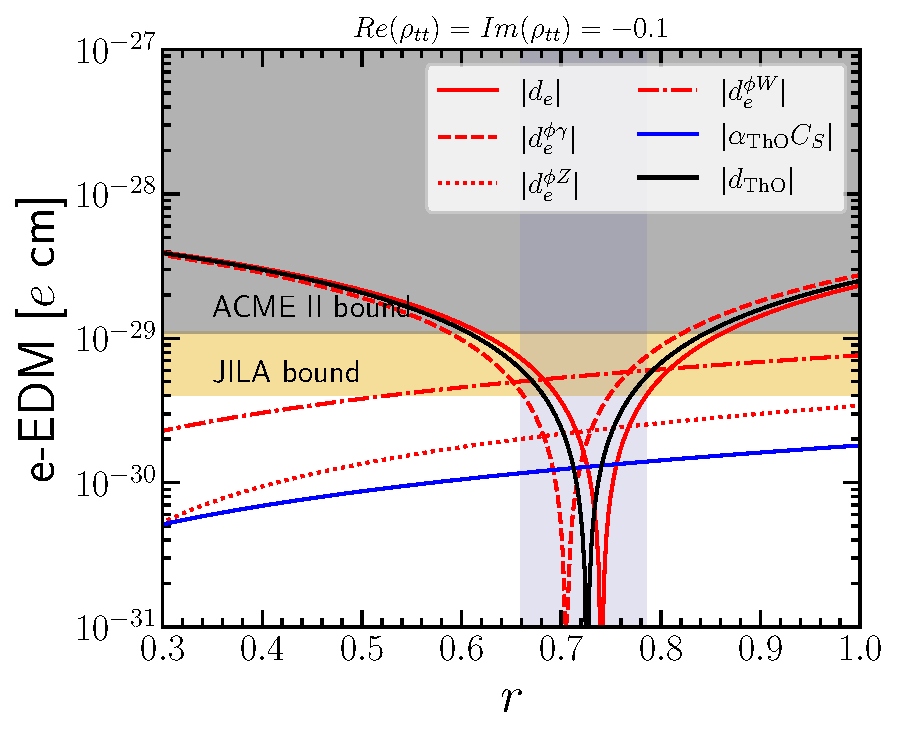
\includegraphics[width=7.95cm,height=5.55cm,angle=-90]{fig2_1.pdf}\\
    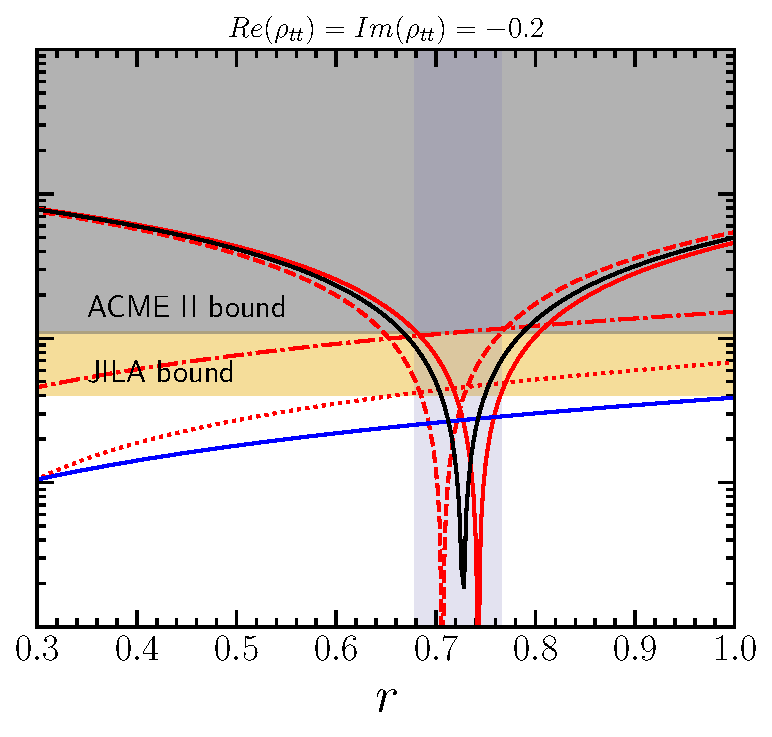
\includegraphics[width=6.95cm,height=5.55cm,angle=-90]{fig2_2.pdf}\\
    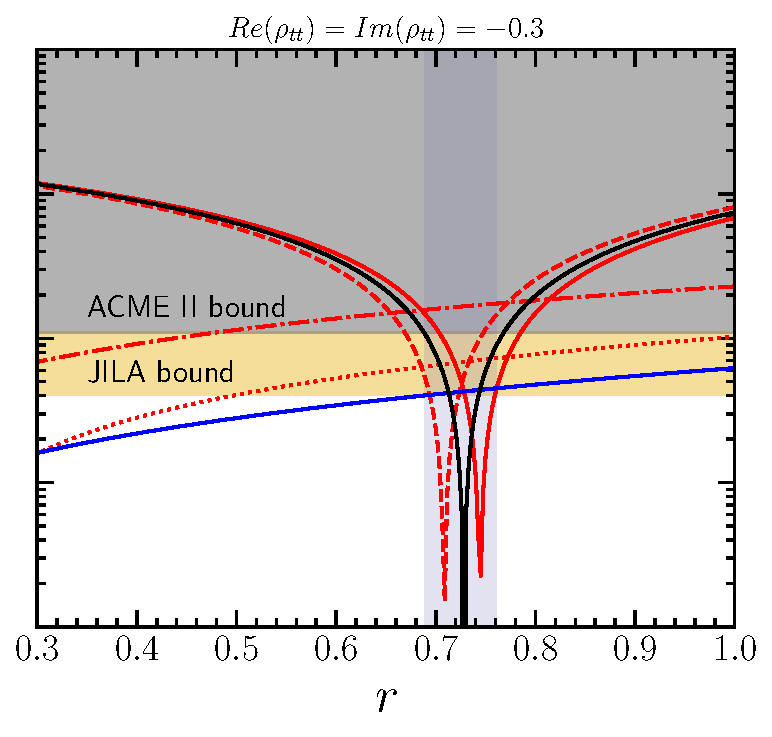
\includegraphics[width=6.95cm,height=5.55cm,angle=-90]{fig2_3.pdf}
    \caption{eEDM v.s. \(r \) for a larger range of \(\rho_{tt} \) with ansatz~Eq.~\eqref{eq:ansatz-extended}. (\(c_{\gamma} = 0.1, m_{H, A, H^+} = 500\,\mathrm{GeV} \))}
    \label{fig:eEDM}
\end{figure}

For the sake of clarity, we have taken a slight liberty in illustrating the range of the purple ``allowed window'' band,
using the left- and right-most curves instead of the left and right side of a given curve.
Nevertheless, the trend we wish to describe is not affected by such.
From our results, it can be seen that as \(|\rho_{tt}| \) increases, the allowed window of the proportionality parameter \(r \) shrinks, yet there is still a decent range of acceptable probable values.
\(\Re\rho_{tt} = \Im\rho_{tt} = -0.1 \) was indeed a conservative representative value, and \(\Re\rho_{tt} = \Im\rho_{tt} = -0.3 \) may still be a viable option in the baryogenesis parameter space.

\section{The Muon}
After the electron, we move on to its slightly heavier cousin, the muon. 
Since the bound on the muon is not as strong, one does not need to resort to the cancellation ansatz immediately.
Instead, we perform a scan of the \(\rho_{tt} \) parameter space for a representative \(\rho_{\mu\mu} \) value, and see how it affects the \(\mu \)EDM.
Results are shown in \figref{muEDM}.

\begin{figure}[p]
    \centering
    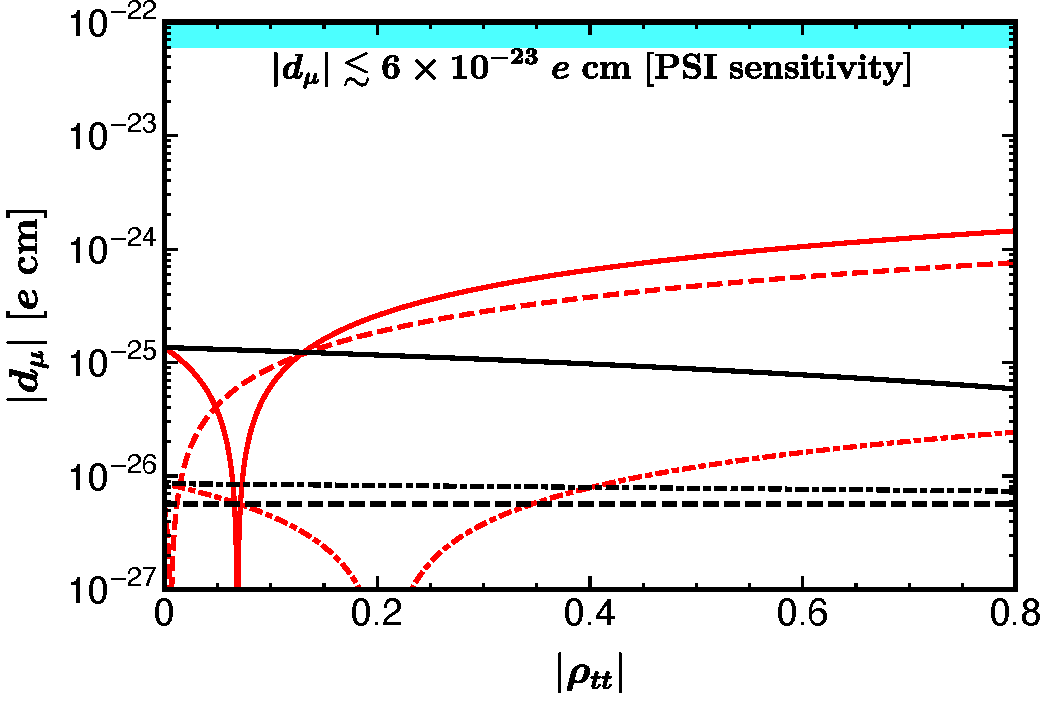
\includegraphics[width=0.7\textwidth]{muEDM.pdf}
    \caption{\(\mu \)EDM results.}
    \label{fig:muEDM}
\end{figure}

We see that there is still a ``cancellation dip'' for the neutral scalar-attached loops, which arises from the opposite signs of the \(W \)-loop and the top-loop.
The details of said cancellation is exactly the same as that of the electron.
Our predicted values for \(\mu \)EDM are still two to three orders of magnitude below the current bounds, so we are eager to see development on the experimental front.
Once the bounds close in, it may also be fruitful to consider the ``cancellation ansatz'' on the muon as well, especially since the leptons share a extra Yukawa matrix \(\rho^{l} \),
which makes it more likely that the \(\rho_{ll} \) might exhibit similar relationships with \(\rho_{tt} \).

\section{The Tau Lepton}
\begin{figure}[p]
    \centering
    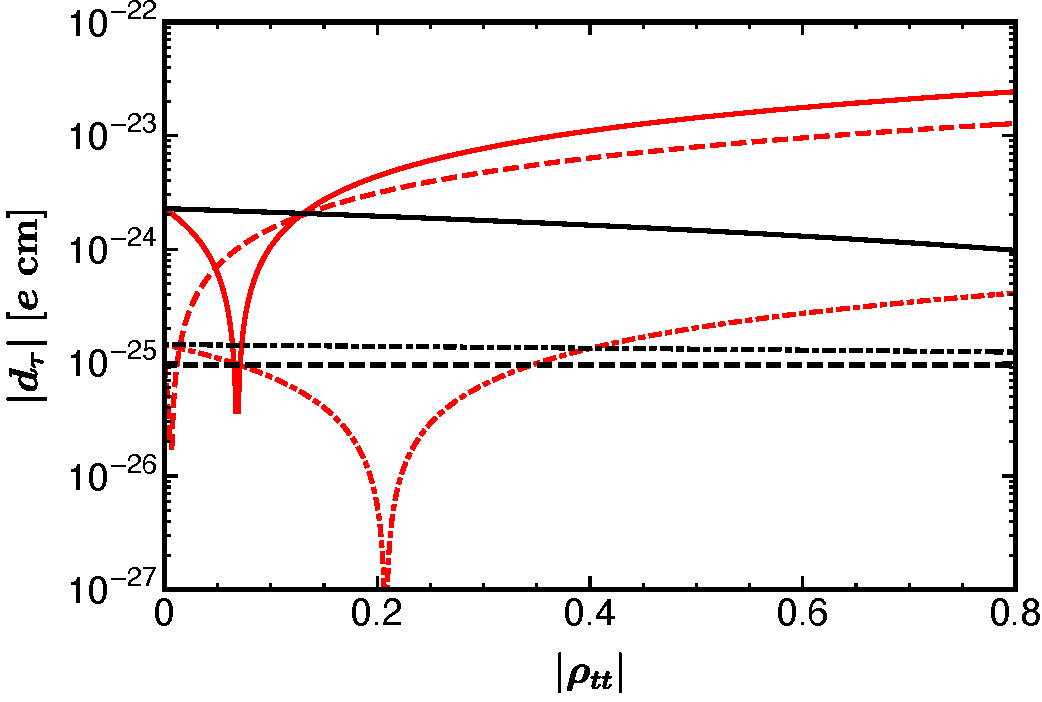
\includegraphics[width=0.7\textwidth]{tauEDM.pdf}
    \caption{\(\tau \)EDM results.}
    \label{fig:tauEDM}
\end{figure}
Lastly, we analyze the heaviest lepton, the tau. 
On the experimental front, the precision of tau EDM (\(\tau \)EDM) measurements are still pretty low.
We perform the same calculations as the muon, with \(\rho_{\mu\mu} = i\lambda_{\mu} \) replaced by \(\rho_{\tau\tau} = i\lambda_{\tau} \).
Results are shown in \figref{tauEDM}.
As seen in the figure, our predicted values are still several orders of magnitude below current experimental results.
Further precision or methodology improvements are required for a more fruitful analysis of \(\tau \)EDM, so we just present our results here without much further comment.

\chapter{Electric and Chromo-electric Dipole Moment of Quarks}
\label{ch:quark(C)EDM}

After the analysis for leptons, we turn our gaze towards EDMs involving quarks. 
However, since quarks are always confined as hadrons, it is extremely difficult, if not outright impossible, 
to directly probe the EDMs of individual quarks, given the state of current technology and our understanding of QCD.
A quick literature~\cite{PDG2022} review shows that there are indeed no direct experimental observations for the EDMs of all the quarks lighter than the top quark.
We comment on the situation of the top quark in \secref{sec:top-cedm}. 
It is natural, under these circumstances, to shift our attention towards hadron EDMs, and utilize the EDM of hadrons to observe the effect of the EDMs of individual quarks.
The prime candidate in this case would be the neutron EDM (\nedm).

\section{The Neutron}
\subsection{Experimental Overview}
Neutron EDM measurements have been in the experimental realm for quite some time already.
The most recent results are given by PSI~\cite{PSI2020nEDM} in 2020, setting the bound at \(|d_{n}| < \num{1.8e-26} \ecm\).
We can use the same back-of-the-envelope mass-scaling estimate that we did for the leptons to estimate the ``equivalent precision'' bound for {\nedm} from the {\eedm} bound.
Since \(m_{u} \sim m_{e} \) and \(m_{d} \) is barely 10 times greater than \(m_{e} \), 
we can place the estimated {\nedm} value at
 \(\sim \num{e-29} \ecm\).
This places the current {\nedm} bound  3-4 orders of magnitude away.

Even though the {\nedm} experimental precision is not as good as that of the {\eedm} experiments,
just looking at the numbers does invoke a \emph{mild} sense of optimism,
especially since this is a \emph{very} naive estimate,
as the dynamics involved in the neutron is much more complicated.
One can reasonably expect the value to be suitably larger.
Unfortunately, that optimistic feeling is quickly extinguished when we take a look at the progress over the past years.
We cite here \figref{fig:snowmass}, taken from the Snowmass conference report~\cite{Snowmass2022EDM}, as a good visual description of {\nedm} experimental progress.
% Figure: Snowmass nEDM experimental status
As can be seen from said figure, progress on the {\nedm} front has stagnated for a decade or so,
with the precision plateauing at \(\sim 10^{-26} \ecm\).
However, we see a silver lining in the report: projects to improve the sensitivity, based on ultra-cold-neutron (UCN) methods, are already in the works.
There is a follow-up project at PSI, named n2EDM~\cite{PSI2021n2EDM}, 
which plans to reach a sensitivity of \(\sim \num{e-27} \ecm \) within a decade.
Furthermore, there is a new experiment under construction at the Spallation Neutron Source~\cite{ORNLnEDM} at Oak Ridge National Laboratory (ORNL),
which projects a precision down to \(\num{e-28} \ecm \).
Nevertheless, it is still worth to explore the {\nedm} parameter space, 
which is what we did~\cite{HKT2024eEDMnEDM}.

\subsection{{\gthdm} Calculations}
As mentioned in the theory section, there are additional chromo-EDM and Weinberg term contributions to take into account that arise from the fact that quarks interact via QCD.
To evaluate the combined combination of these contributions to {\nedm}, we use the more recent formula~\cite{Hisano2014nEDM}
\begin{equation}
  d_n = - 0.20\,d_u + 0.78\,d_d + e\,(0.29\,\tilde d_u + 0.59 \tilde d_d) + e\,23\;{\rm MeV}\,C_W
\end{equation}
instead of the widely cited classic review of Pospelov and Ritz~\cite{PospelovRitz2005EDMs}.
We present the {\gthdm}-with-extended-ansatz~\eqnref{eq:ansatz}-applied calculation results for {\nedm} in \figref{fig:nEDM-fixed}.
% Figure: nEDM results
Interestingly, our predictions for {\nedm} are not too far below the current experimental bound.
We see that, even for \(|\rho_{tt}| = 0.3\sqrt{2} \approx 0.42\), one can still survive the current PSI bound.
The projected \(\sim \num{e-27} \ecm \) sensitivity of n2EDM at PSI covers the range illustrated in \figref{fig:nEDM-fixed},
putting stress on our model.
Fortunately, there is still a possibility of lowering the predicted {\nedm} value of our model 
should the new experimental bounds indeed close in.

So far, we have been utilizing the ``extended'' cancellation ansatz~\eqnref{eq:ansatz-extended} in our above calculations and analyses.
However, we have to reiterate that it is merely a convenient way to numerically illustrate the \textit{flavor hierarchy} of the {\gthdm}.
A closer examination of the ``extended'' ansatz reveals a logical flaw: 
since \(\rho_{uu} \) and \(\rho_{tt} \) are in the same \(\rho \) matrix, and the ansatz obviously does not hold for \(\rho_{tt} \) itself, 
there is no reason to expect it to hold for \(\rho_{uu} \).
Thus, for this situation, we should fall back one step, and rely on the \textit{rule of thumb}~\eqnref{eq:ruleofthumb} instead of the ansatz.
Hence, we relax the ansatz for \(\rho_{uu} \), and explore the range of \(\order{\lambda_{u}} \) by varying
\begin{equation}
  |\rho_{uu}| \in [0.3\lambda_u, 3\lambda_u], \quad \arg\rho_{uu} \in [-\pi, \pi]
\end{equation}
while keeping the other \(\rho_{ff} \)s intact, i.e. still following the ansatz.
We present our results for said variation in \figref{fig:nEDM-varied}.
% Figure: nEDM varying rho_uu
The different colors of the points represent different values of \(\arg\rho_{uu} \), and an interesting pattern can be seen among them.
The red points have negative \(\arg\rho_{uu} \), which is the same sign as \(\rho_{tt} \); 
the {\nedm} of these points are larger, but stay mostly below the PSI bound.
On the other hand, the blue points have \textit{positive} \(\arg\rho_{uu} \), which is the \textit{opposite} sign as \(\rho_{tt} \); 
remarkably, the value of {\nedm} of these points drop significantly, reaching as low as \(\num{e-28} \ecm \) or lower, 
evading even the projected sensitivity of n2EDM!
This phenomenon in \figref{fig:nEDM-varied} illustrates a \textit{natural} cancellation mechanism present within the dynamics of {\nedm},
arising from the phase difference of \(\rho_{uu} \) and the other \(\rho_{ff} \).
Even though this mechanism can evade the projected n2EDM sensitivity, 
it can still be probed by the SNS at ORNL, with its down to \(\sim \num{e-28} \ecm \) projected sensitivity.
This experiment may take more than a decade to come to fruition, but it almost fully covers our projected range, since the blue dots are still mostly concentrated above \(\num{e-28} \ecm \).

\clearpage
% Snowmass nEDM experimental status
\begin{figure}[p]
    \centering
    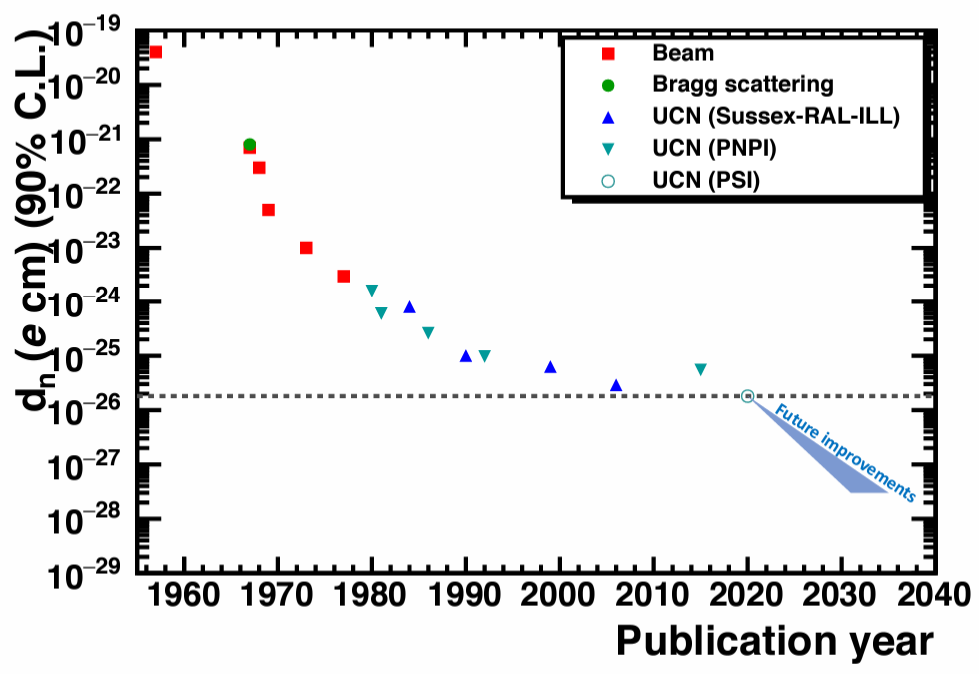
\includegraphics[width=0.5\linewidth]{Snowmass_fig.png}
    \caption{nEDM experimental progress~\cite{Snow22}}
    \label{fig:snowmass}
\end{figure}

% nEDM fixed rho_uu
\begin{figure}[p]
    \centering
    \begin{minipage}{0.48\textwidth}
      \centering
      \includegraphics[width=0.85\linewidth]{example-image}
      \caption{nEDM results.}
      \label{fig:nEDM-fixed}
    \end{minipage}\hfill
    \begin{minipage}{0.48\textwidth}
      \centering
      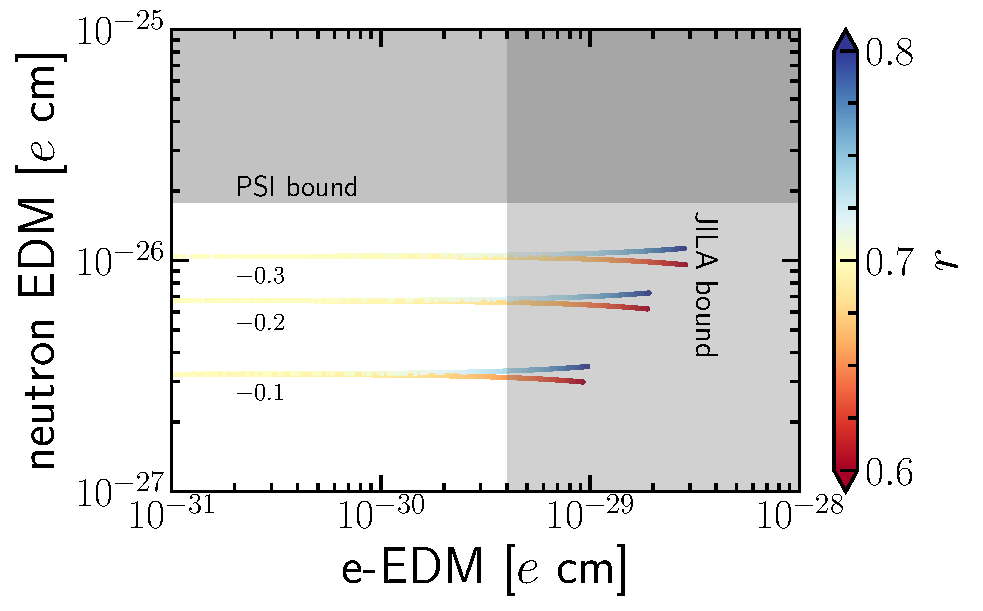
\includegraphics[width=0.95\linewidth]{fig3.pdf}
      \caption{Combined eEDM-nEDM result.}
      \label{fig:nEDM-eEDM}
    \end{minipage}
\end{figure}

% nEDM varying rho_uu
\begin{figure}[p]
    \centering
    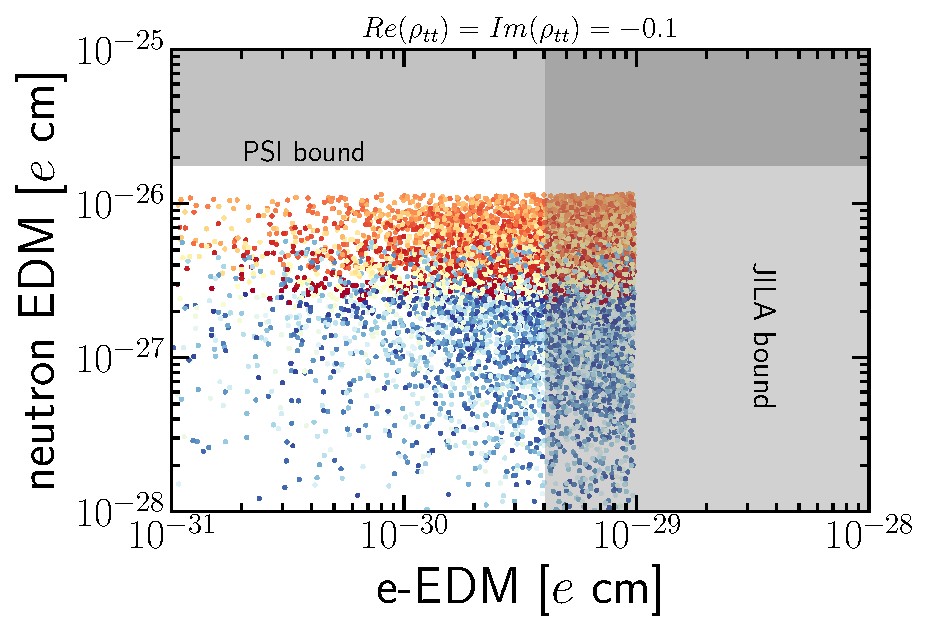
\includegraphics[width=7.35cm,height=5.55cm,angle=-90]{fig4_1.pdf}\\
    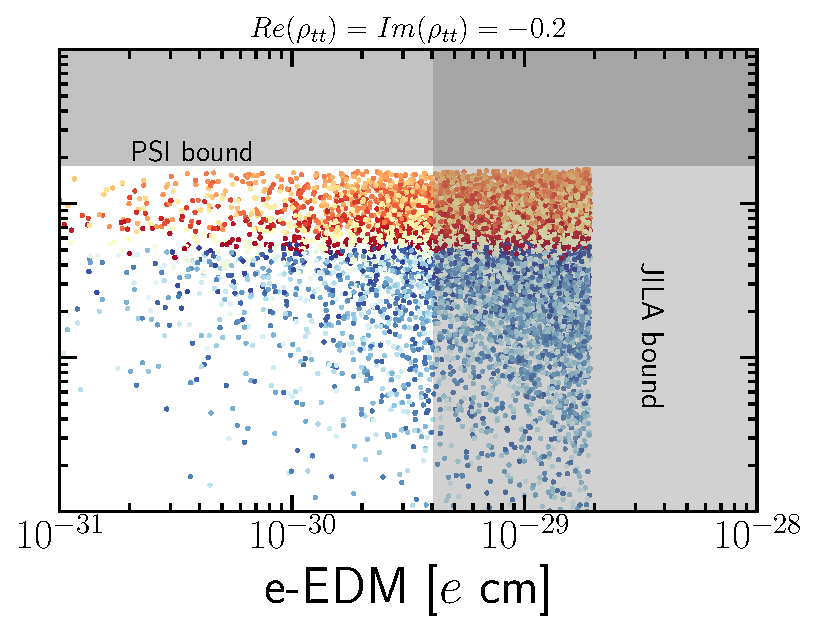
\includegraphics[width=6.45cm,height=5.55cm,angle=-90]{fig4_2.pdf}\\
    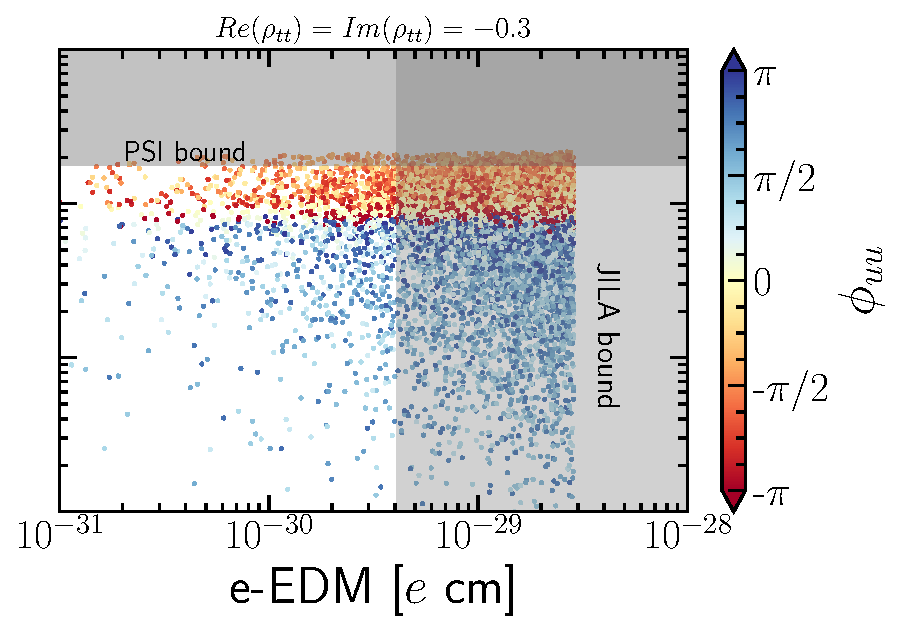
\includegraphics[width=7.89cm,height=5.55cm,angle=-90]{fig4_3.pdf}
    \caption{Results for eEDM and nEDM with \(|\rho_{uu}| \sim \lambda_{u}\).}
    \label{fig:nEDM-varied}
\end{figure}
% \chapter{(Semi-)Leptonic \(B \) Meson Decays}
\label{ch:leptonic_B_decays}
Something something \(B_{s} \to ll \), cf. our 2023 paper.

\chapter{Conclusion}
\label{ch:conclusion}
\section{Comments}
Before we reach the summary of this study, we want to comment on some unaddressed details.

\subsection{Heavy Higgs Masses}
Throughout the calculations in this study, we have assumed degeneracy of the exotic Higgses, either at 300 or 500 GeV.
This has been done primarily to reduce the number of variables in the analysis, and focus on the effects of the extra Yukawa couplings on various EDMs.
As a matter of fact, this assumption is actually two assumptions in one: the choice of benchmark mass value and the choice of imposing degeneracy.
We would like to address the concequences of lifting/flexing each assumption seprately.
First, regarding the choice of benchmark.
For eEDM and nEDM, we have set the exotic Higgs masses to the higher value of 500 GeV.
This leads to a smaller two-loop contribution to the EDMs, since the loop functions are dependent on and monotonically increasing with \(m_{t/W}^{2}/m_{H/A/H^{+}}^{2} \).
This also changes the exact \(r \) value where the cancellation occurs.
However, at the same time, larger exotic Higgs masses lead to a less efficient scenario for baryogenesis.
In a sense, this is the ``conservative'' benchmark, sacrificing baryogenesis efficiency for some extra ``headroom'' in evading the EDM bounds.
On the other hand, the 300 GeV mass value used in the \(\mu \)EDM and \(\tau \)EDM calculations is the ``optimistic'' benchmark,
meant to explore the upper limits of the respective EDMs and see how close we are to the current experimental bounds.
We have checked the eEDM and nEDM calculations at the 300 GeV benchmark and, unsurprisingly, the qualitative results are the same, with only the quantitative differences described above.
Second, regarding the mass degeneracy.
As mentioned in~\secref{g2hdm_in_edm}, with the degeneracy in place, one-loop effects are even further supressed.
Lifting this degeneracy will increase the importance of the one-loop contribution, but unless the off-diagonal terms of the lepton \(\rho \)-matrix are large,
which runs against our \textit{flavor hierarchy} phenomenon, 
the two-loop effects will still be dominant by at least an order of magnitude or two.
Also, nondegenerate exotic Higgs masses opens us up to the scrutiny of electroweak precision constraints~\cite{PDG2022}.
This will require us to explore the scenarios of custodial symmetry \(m_{A} = m_{H^{+}} \) and twisted-custodial symmetry~\cite{Gerard2007TwistedCustodial} \(m_{H} = m_{H^{+}} \).
All in all, we can still enlarge the parameter space by varying the masses of the exotic Higgses, but we will have to deal with different constraints.
We thus relegate a thorough investigation of the Higgs masses to further studies.

\subsection{Muon \(g-2 \)}
During our analysis of \(\mu \)EDM and \(\tau \)EDM, the Fermilab Muon g-2 experiment reported~\cite{Fermilab2021MuonGminus2} their first measurement of the muon anomalous magnetic moment \(a_{\mu} = (g-2)_{\mu} \).
Their result not only confirmed the old BNL result~\cite{BNL2006MuonGminus2}, but also put the combined experimental value at \(a_{\mu}^{\text{Exp}} = \num{116592061(41)e-11} \),
which disagreed with the SM prediction~\cite{Aoyama2020MuonTheory} \(a_{\mu}^{\text{SM}} = \num{116591810(43)e-11} \) by more than \(4\sigma \),
\begin{equation}
    a_{\mu}^{\text{Exp}} - a_{\mu}^{\text{SM}} = (251 \pm 59) \times 10^{-11}.
\end{equation}
This was indeed a shock at that time, which prompted us to add in related discussions and analysis to our EDM study.
As it is not the main point of \textit{this} study, we refer you to section V of our paper~\cite{HKT2022MuonEDMTauEDM} for detailed discussion, with a brief summary given here.
Muon \(g-2 \) has main contributions in {\gthdm} from the one-loop diagram, so to accomodate the experimental result, 
one needs~\cite{HouEtal2021Muon} very large \(\rho_{\tau\mu} \) and \(\rho_{\mu\tau} \), as well as sub-TeV \textit{nondegenerate} \(m_{H} \) and \(m_{A} \).
This implies a near-perfect alignment \(c_{\gamma} \to 0\) and a small \(\rho_{tt} \).
This in turn suppresses the two-loop contributions to all EDMs, while also makeing baryogenesis less favorable.
Although the most recent experimental update~\cite{Muon2023Gminus2} on this matter has strengthened the precision of the 2021 result, 
the other fronts do not look as optimistic.
Recent lattice QCD results~\cite{Borsanyi2021Lattice} are in tension with other relevant experimental results~\cite{CMD32023eetopipi};
meanwhile, theorists are attempting~\cite{Colangelo2022Gminus2theory} to reconcile the current theoretical situation.
It remains to be seen how this ``anomaly'' will develop in the future.

\subsection{Top Chromo-EDM}\label{sec:top-cedm}
We would like to mention that the nEDM portion of this study was originally motivated by the ability of the LHC to probe top CPV through top chromo-EDM~\cite{CMS2023}.
Probing the EDM and cEDM of the top quark directly would be ideal for direct exploration of the \(\rho_{tt} \) parameter space.
Alas, the current bounds of the top cEDM are still relatively weak, so we shifted our gaze towards other hadronic EDMs and settled on nEDM, 
where the up and down cEDM come into play.
Fortunately, we found rather good prospects for {\gthdm} in nEDM!
We do hope that future improvements on the top cEDM measurement will come to fruition,
and eagerly anticipate the insights it may bring in the realm of CPV and BAU.

\section{Summary and Conclusion}
In this thesis, we have analyzed various EDMs of fundamental particles in the framework of  the General Two Higgs Doublet Model,
a two-Higgs doublet model characterized by lack of \(Z_{2} \) symmetry, \textit{alignment} between the SM and exotic Higgs, and extra Yukawa couplings governed by \textit{flavor hierarchy}.

We note that to evade precision bounds while satisfying the conditions for baryogenesis, a cancellation is possible,
which is also an indicator of an underlying \textit{flavor hierarchy}.
This is most prevalent in eEDM, where bounds are the strongest, and experimental precision improving rapidly.
We analyze \(\mu \)EDM, with our predictions still being a couple orders of magnitude below current experimental bounds.
We present results for \(\tau \)EDM, but provide no further analysis since the bounds are still too imprecise.
We analyze quark EDM through nEDM, and optain promising prospective results, especially when viewed together with eEDM.
We stress that this is a noteworthy area to pay attention to in the upcoming decade or two.

The improved precision of the eEDM and nEDM experiments may shake up new discussion in the realm of CPV.
Along with direct searches for exotic Higgs at LHC, ongoing efforts at Belle II as well as other flavor frontiers,
we might soon see whether we can unveil what Nature has laid out for baryogenesis.
\end{fmffile}

%------------------------------------
% Thesis Body -- end
%------------------------------------

\bibliographystyle{IEEEtran-mod}
\bibliography{thesis}
\end{document}
